\section{Otros protocolos multimedia}

\subsection{Miracast}
Miracast es un protocolo multimedia para hacer streaming a un monitor desde un dispositivo local. Para que nuestra smartTV sea capaz de usarlo, necesita soportar Wi-Fi Direct. Wi-Fi Direct es una norma que permite la conexión entre dos dispositivos Wi-Fi sin necesidad de un intermediario.
Los dispositivos que envían y reciben información tienen que estar certificados para Miracast, pero existe un plug para dispositivos no certificados.
Miracast está disponible de manera nativa para dispositivos con versiones de Android 4.2 y Android 6.0.

\vspace{0.1cm}
\begin{figure}[ht]
	\begin{minipage}[b]{0.55\linewidth}
		La conexión está creada vía Wi-Fi Protected Setup (WPS), mecanismos para facilitar la configuración de una red WLAN con seguridad WPA2.
		WPS contempla cuatro configuraciones para el intercambio de credenciales: PIN (Personal Identification Number), PBC (Push Button Configuration), NFC (Near Field Communications) y USB (Universal Serial Bus). La configuración PIN no es recomendable por su debilidad ante ataques de fuerza bruta.
	\end{minipage}%%
	\begin{minipage}[b]{0.45\linewidth}
		\centering
		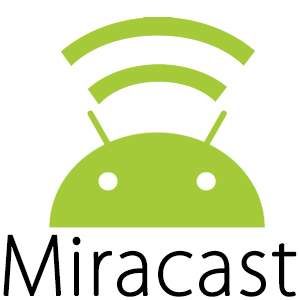
\includegraphics[width=.55\linewidth]{./Imagenes/miracast.jpg}
	\end{minipage}
\end{figure}

\

Para la capa de internet usa IPv4; para la de transporte, TCP/UDP, y para la de aplicación, RTSP y RTP, que se encargan de controlar el streaming.

\

A partir de Android 6.0, Google ha dejado de dar soporte nativo a Miracast en favor de su propio Google Cast.
Con Miracast el dispositivo receptor es dependiente de que el dispositivo Android emisor se mantenga activo \cite{Miracast}: si se bloquea también bloqueará la reproducción en el receptor.
Esto implica una mayor carga de trabajo y consumo de batería respecto a Google Cast, que solo se encarga de enviar señales para el control de la reproducción.

\

Existe una alternativa de código abierto a Miracast llamada MiracleCast. El nombre viene por la dificultad de crear una red Wifi-P2P estable (basado en wpa\_supplicant).

\

El núcleo de MiracleCast es un demonio llamado miracled \cite{MiracleCast}, que controla links locales, las peticiones de conexión, se encarga de la codificación del protocolo y el parsing.
Su línea de comandos puede ser usada para controlar el demonio, crear nuevas conexiones, modificar parámetros, etc.
Soporta un modo interactivo que muestra las peticiones de conexión y permite al usuario aceptarlas o no.

\

El código fuente se puede encontrar en \href{https://github.com/albfan/miraclecast}{GitHub}.
